La construcción de un modelo semántico sobre un dominio de negocio concreto
consiste en el desarrollo de un sistema de conocimiento que describa las
entidades y propiedades, así como las relaciones lógicas que existen entre
las mismas. Un aspecto, muchas veces minusvalorado, es que en estos modelos de
dominio es necesario describir también los procesos, las restricciones y en
general, los aspectos dinámicos del dominio. Este tipo de modelos formalizados
mediante un lenguaje lógico, como ya se ha descrito, se denominan ``ontologías''. La selección de la lógica apropiada para la modelización de 
la base de conocimiento no es una cuestión sencilla y se deberán contemplar diferentes
factores tales como grado de computabilidad, decidibilidad, soporte razonadores, etc. Existen
diferentes vocabularios y lenguajes que permiten modelar un cierto dominio, algunos
de los cuales ya se han repasado (\gls{RDF}, RDFS, \gls{OWL} y \gls{WSML}) en la Sección~\ref{sect:arch-ws}, no obstante, existen otros estrechamente
ligados a entornos de negocio, que a continuación se presentan.


\begin{description}
\item[\gls{RIF} (\textit{Rule Interchange Format})~\cite{rif-core}.] RIF constituye una familia de lenguajes con diferente expresividad, 
cuyo objetivo es convertirse en \textit{lingua franca} para el intercambio de
conocimiento basado en reglas en la Web. Define la compatibilidad con
documentos RDF y OWL, además está especialmente diseñado para integrarse con
sistemas de inferencia basados tanto en reglas de producción, como de
Programación Lógica. La ventaja de RIF respecto de OWL es una mayor expresividad, 
que permite expresar conocimiento causal y procedimental. 


\item [\gls{SCOR} Model (\textit{Supply-Chain Operations Reference-Model}).] Es un modelo conceptual de
referencia para la especificación y formalización de los procesos de negocio
asociados a las cadenas de suministro. Este modelo define los procesos de
planificación, fabricación, entrega, evolución e inventarios de productos en una
cadena logística.

\item [\gls{SBVR} (\textit{Semantics of Business Vocabulary and Business Rules}).] Es un estándar
(ISO 704/1087) desarrollado por el \textit{Object Management Group} (\gls{OMG}). Define un
metamodelo para el desarrollo de modelos semánticos de vocabularios y reglas de
negocio. La idea es que a partir del lenguaje natural se puedan expresar
vocabularios y reglas de negocio en un dominio concreto. La construcción de un
modelo de negocio mediante el SBVR recoge el vocabulario de conceptos del
dominio y la definición de lógica formal asociada.

\item [Clasificaciones de productos de comercio electrónico~\cite{Leukel-ecatalog2005,Leukel-standard,Leukel-automating}.] Para
facilitar el intercambio automático de información y la anotación de los diferentes productos
y documentos que forman parte del comercio electrónico, distintos sectores de
actividad económica han desarrollado sus propias terminologías o
vocabularios~\cite{Norbert-class} controlados, para armonizar mediante códigos unívocos la identificación de
los objetos de negocio. Ejemplos de estos vocabularios son: el estándar eCl@ss o
la clasificación \gls{UNSPSC} entre otros, ver Sección~\ref{sect:pscs}.


\item [\gls{ebXML} (\textit{Electronic Business using eXtensible Markup Language}).] Es un lenguaje
\gls{XML} elaborado por \gls{OASIS} y UN/CEFACT, también consta de una infraestructura que permite la comunicación entre entidades
participantes en transacciones de negocio electrónico, favoreciendo la interoperabilidad y la seguridad de una forma homogénea entre las distintas partes.
La propuesta original cubría cinco capas: \textit{Business processes}; \textit{Collaboration protocol agreements};
\textit{Core data components}; \textit{Messaging} y \textit{Registries and repositories}.

eBXML ha sido aprobado por \gls{ISO} en un conjunto de especificaciones, ISO 15000:  ISO 15000-1: ebXML \textit{Collaborative Partner Profile Agreement};
ISO 15000-2: ebXML \textit{Messaging Service Specification}; ISO 15000-3: \textit{ebXML Registry Information Model}; ISO 15000-4: ebXML \textit{Registry Services Specification};
y ISO 15000-5: ebXML \textit{Core Components Technical Specification}, Version 2.01.

\item [\gls{XBRL} (\textit{extensible Business Reporting Language}).] 
Es una norma elaborada en el año 1998 por Charles Hoffman, contable y auditor, para
simplificar la automatización del intercambio de información financiera mediante
el uso del lenguaje XML. La familia de lenguajes XBRL se ha realizado para
satisfacer las exigencias principalmente de información financiera y
empresarial, permite aplicar etiquetas identificativas multilenguaje con
significado, por ejemplo indicando si es un valor monetario, también es posible
mostrar la relación que guardan los elementos entre sí, así se podría saber cómo se
calculan. Una característica muy importante es la capacidad de extensión, de
esta forma es capaz de adaptarse para casos particulares de empresas. 

\end{description}

\subsection{Actividades de aplicación de Semántica en \textit{e-Procurement}}
Desde la creación del movimiento de la Web Semántica, en concreto de la realización
práctica mediante \linkeddata, se han aplicado los principios de estas iniciativas a múltiples
dominios como ya se ha reseñado en las secciones anteriores. Evidentemente en un sector como 
la Administración Pública, caracterizado por su amplitud, casuística y carácter estratégico para todos los ciudadanos
es por lo que la semántica y sobre todo las corrientes de \opendata y \linkeddata han penetrado con mucha fuerza en los últimos años. 
En un principio los esfuerzos como en otros dominios, se centraban en el modelado de la administración
como organización y de sus procesos, con el objetivo de mejorar la interoperabilidad e integración
entre las aplicaciones y facilitar los trámites burocráticos. En muchos casos se han desplegado
soluciones flexibles basadas en la reutilización de información, procesos y conocimiento a través
de grandes bases de datos compartidas, servicios web y sistemas basados en reglas, no obstante la inmersión
de la semántica propiamente dicha se centraba en la realización de modelos para formalizar
cuestiones relativas a documentación y a procesos administrativos. Por ello,
la irrupción de \opendata y \linkeddata ha reorientado el esfuerzo de las Administraciones Públicas
para aprovechar la semántica en su beneficio. 

Por otra parte, también han surgido iniciativas~\cite{DBLP:journals/tcci/Alor-HernandezAJPRMBG10} relacionadas con \eproc, pero desde un punto de vista
de las cadenas de suministro, en las cuales se modelan de forma completa un entorno de proveedores y suministros mediante la coordinación
de los recursos software, hardware y humanos propios de un entorno de este tipo, como son \gls{ERP}s, robots o las propias personas. 

\subsubsection{Ontología de Contratos Públicos del proyecto LOTED}
El diseño de la ontología en el proyecto LOTED~\cite{loted-project}, es de suma importancia debido a su consideración 
como primer gran esfuerzo por aunar las iniciativas de \linkeddata y \opendata en el campo de la contratación 
pública electrónica. En este proyecto la propuesta principal consiste en la transformación directa 
de la información proveniente del \gls{RSS} de \gls{TED} a \gls{RDF} para su posterior indexado en un repositorio y acceso 
mediante un \textit{endpoint} de \gls{SPARQL}. Como sucede un muchos casos relacionados con la iniciativa 
de \linkeddata la ontología realizada, ver Figura~\ref{fig:public-contracts-ontology-loted}, está orientada a la representación de los datos en sí, estableciendo 
un modelo formal en el cual enclavar los recursos RDF generados, pero si bien este enfoque es válido, tan sólo 
representa una parte de la casuística presente en el dominio de la contratación pública electrónica. El intento 
realizado en TED se centra en el diseño de las entidades presentes en la información del RSS para así suministrar 
un modelo formal a los recursos RDF. Por todo ello, esta ontología sirve como una gran fuente de información 
para comprobar que tipo de entidades se recogen o publican en el RSS de TED, pero en un espectro más amplio 
se considera insuficiente para la representación de información teniendo en cuenta los modelos de datos 
disponibles en las plataformas de contratación o el propio de \gls{opXML} realizado en el proyecto ``10ders Information 
Services'', como ha quedado señalado en la Sección~\ref{data-model-eproc}. 

Por otra lado y desde el punto de vista del acceso a los datos, se ofrece la posibilidad de la realización 
de consultas en SPARQL seleccionando una serie de códigos y acotando los resultados por fechas, sin embargo este sistema 
parece desactualizado y no se han realizado cambios en los últimos dos años. 

\begin{figure}[h]
 \centering
    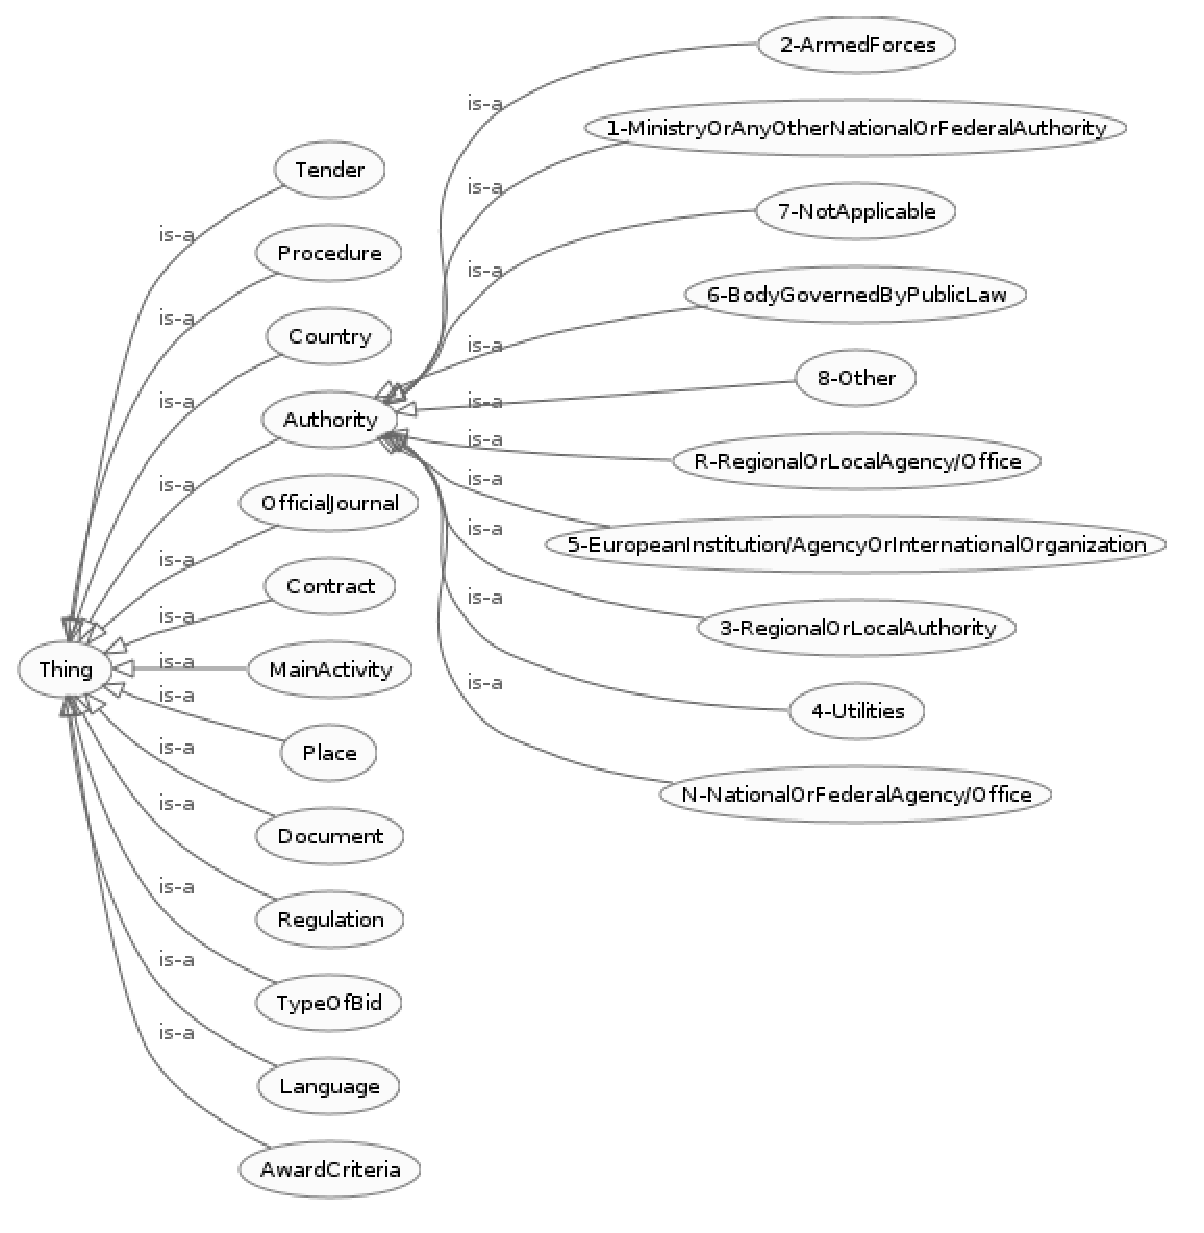
\includegraphics[width=14cm]{images/phd/loted-ontology}
  \caption{Ontología de Contratos Públicos del proyecto LOTED.}
 \label{fig:public-contracts-ontology-loted}
\end{figure}

\subsubsection{Ontología de Contratos Públicos de la República Checa}
Esta ontología está siendo desarrollada por el grupo \textit{Knowledge Engineering Group} 
de la \textit{Charles University} de Praga en la República Checa. Parte del esfuerzo está siendo
cubierto parcialmente dentro del proyecto europeo LOD2 en su paquete de trabajo \textit{WP9A – LOD2 for a Distributed Marketplace for Public Sector Contracts}, cuya descripción es la siguiente:

\begin{Frame}
\textit{The objective of this use case is to explore and demonstrate the application of linked data principles for procuring contracts in the public sector...}
\end{Frame}

Este trabajo enlaza perfectamente con el propósito de este documento, esto es cubrir el sector de los contratos
públicos con semántica y concretamente con la iniciativa \linkeddata. Es por ello que se ha establecido
contacto con los integrantes del grupo de investigación de esta Universidad para aprovechar y realimentar
esfuerzos, como fruto de esta colaboración han empezado a reutilizar los códigos CPV, resultado de este trabajo y del proyecto ``10ders Information Services''.

La ontología que se ha desarrollado en este grupo, ver Figura~\ref{fig:public-contracts-ontology}, tiene como intención recoger
la información y datos de los contratos públicos de forma estructurada, para que pueda ser consumida
automáticamente tanto por personas como por máquinas, desarrollándose también dentro del ámbito
de la iniciativa de \opendata de la República Checa. Desde un punto de vista del diseño reutiliza varios
vocabularios y ontologías ya disponibles, como \textit{Payments Ontology} del Reino Unido, lo que confiere a este modelo un carácter integrador y 
reutilizable. No obstante, abordar la descripción de toda la casuística del proceso de contratación pública electrónica parece
muy ambicioso y podría presentar problemas de interoperabilidad, integración y reutilización ya que 
puede estar muy orientada a la problemática de un entorno particular. Otro de los puntos importantes
que se deben abordar, y parcialmente recogidos en esta ontología y que deben servir de guía, están referidos a 
la adición de metainformación para \textit{provenance}, licencia, etc., que si bien en algunos
\datasets es importante, en la información de carácter público es fundamental y debe ser un requisito
para las propias entidades públicas.

\begin{figure}[h]
 \centering
    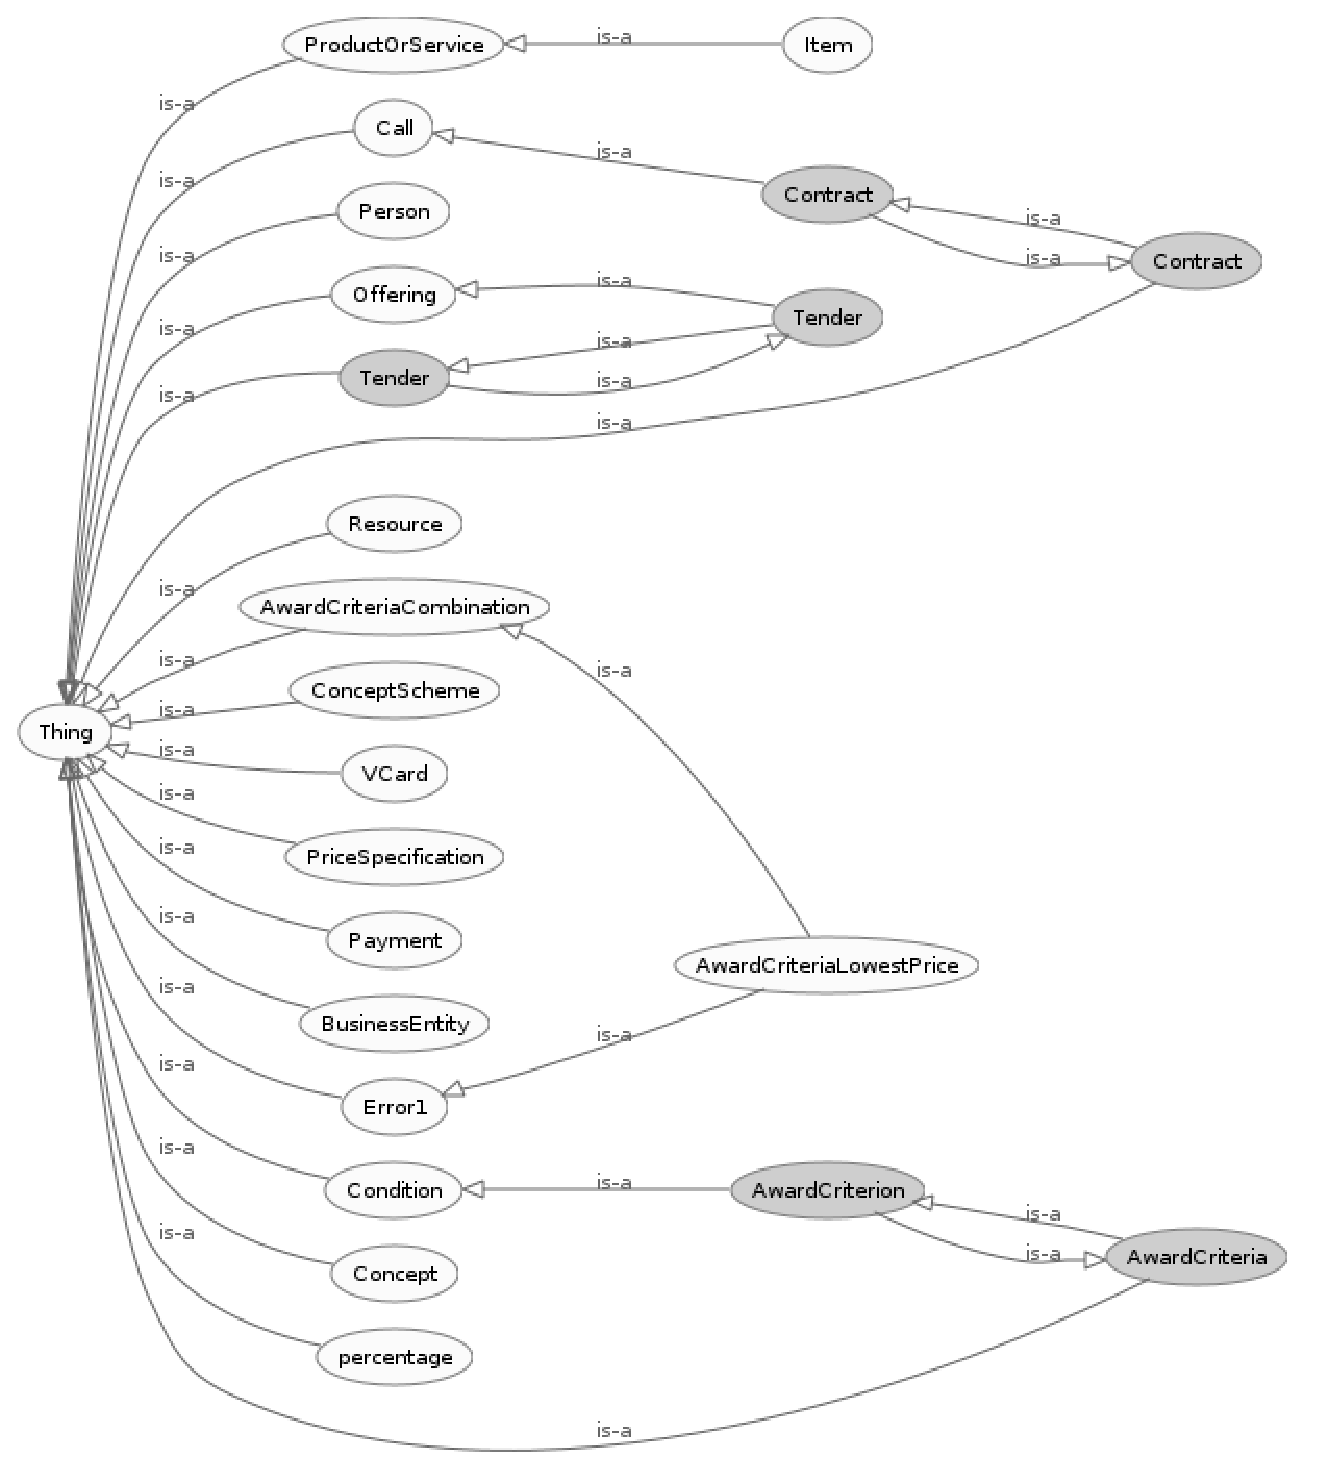
\includegraphics[width=14cm]{images/phd/public-contracts-ontology}
  \caption{\textit{Public Contracts Ontology from Czech Republic.}}
 \label{fig:public-contracts-ontology}
\end{figure}


\subsubsection{Clasificaciones Estándar de Productos}\label{semantica:pscs}
Las clasificaciones de productos, son instrumentos claves de estandarización~\cite{Leukel-standard} que nacen con el fin de
conseguir una clasificación común de productos y servicios. En general, son variadas~\cite{Leukel-ecatalog2005}
y obedecen a intereses particulares dependiendo del sector como e@Class o RossetaNET,
o bien de carácter global como \gls{UNSPSC} u otras destinadas a un dominio particular como el \gls{CPV} en la Administración Pública, ver Sección~\ref{sect:pscs}. Las diferencias
estriban en su alcance y cobertura sectorial, pero también en el grado de especificidad o nivel
de profundidad que existe para describir los productos o servicios.

Como señala Hepp\cite{HeppTrueComplexity,HeppEclass,HeppMethodology} todos estos
estándares reflejan una combinación de componentes variables, que pueden ser
utilizados para la construcción de una ontología derivada a partir de la clasificación.
Sin embargo, se puede identificar una estructura común subyacente a todas ellas y
que es fundamental señalar para proporcionar un modelo de datos semántico universal para este tipo de clasificaciones, consistente 
en que todas estas clasificaciones se ordenan jerárquicamente. 

\begin{description}
 \item [Categorías de productos.] Las clasificaciones se dividen en categorías o
clases de productos, agrupando los distintos elementos del catálogo.
\begin{itemize}
 \item Las categorías de la clasificación se organizan jerárquicamente.
 \item Cada elemento de la clasificación pertenece a una categoría de
productos.
 \item Cada elemento de la clasificación pertenece sólo una categoría de
productos, es decir, las categorías son disjuntas.
\end{itemize}

\item  [Estructura taxonómica.] Además de la división en niveles de jerarquía
de los elementos de la clasificación, su objetivo es organizar y agrupar los productos en
sectores verticales mediante algún tipo de criterio establecido por la comunidad
que desarrolla el estándar. 
 
\end{description}

Estas son características genéricas de las clasificaciones de productos. Sin
embargo, otras clasificaciones más sofisticadas incluyen un diccionario de propiedades
estándar que se puede utilizar para describir productos con más detalle.
Normalmente, estos diccionarios de propiedades también incluyen los tipos de
datos que pueden ser valor de las mismas, así como su referencia con respecto a estándares internacionales para establecer las unidades de medida, este es el caso
de la clasificación de productos de e@Class. En otras ocasiones, se construyen
clasificaciones multiling\"{u}es para la expresión de los descriptores de cada
elemento. 

La irrupción de la tecnología semántica y, sobre todo, la aparición de
lenguajes web para la representación de conocimiento y gestión de metadatos, ha
propiciado un creciente interés en el uso de las clasificaciones estándar de productos para mejorar tanto el
intercambio de información, como su capacidad para estructurar información. La construcción de ontologías de productos 
con alto nivel de detalle implican un coste que es muy difícil de asumir en muchos casos. 
Los autores~\cite{Yu:2009:CSI:1693684.1693743,FenselOmel2001,FenselDing2001} comparten la opinión de Corcho~\cite{CorchoECommerce} 
de que una ontología de productos sería muy útil para la organización conceptual del mercado, se entiende que estas ontologías tienen
más carácter privado, para la organización de la producción, los departamentos
de ventas y comerciales y, en general, para cualquier área de una empresa o
institución que deba tratar con la gestión de productos.

El desafío básico más importante que hay que afrontar cuando se deriva una
ontología de una clasificación de productos, se refiere a cómo interpretar la semántica original de la taxonomía.
No existe una definición formal de las relaciones taxonómicas que construyen
cada categoría de la clasificación y es tentador utilizar la propiedad de un
vocabulario de ontologías, como \textit{rdfs:subClassOf}, para intentar
representar estas relaciones semánticas, sin embargo, esta suposición es errónea. Como señala~\cite{HeppMethodology}, esta relación de jerarquía entre los elementos no se puede considerar
equivalente a una relación de subclase o de herencia. En primer
lugar, tomando el siguiente ejemplo: el elemento ``Partes y accesorios de
bicicleta'' del \gls{CPV} 2008 (34432000-4) tiene como antecesor a ``Bicicletas''
(34440000-0), donde la relación semántica entre los dos elementos no es
herencia, es decir, no se puede expresar que una \textbf{parte de una bicicleta}
sea una \textbf{bicicleta}. Para ser más precisos, debería modelarse como una relación de
composición o agregación. En este sentido, ocurre igual con la relación
taxonómica entre ``Tubos de resina Epoxi''(19522110-5) y ``Resina Epoxi''
(19522100-2), en el que es difícil justificar de nuevo una relación de herencia
clásica entre el primero y el segundo elemento del CPV, ya que en ningún caso
se puede considerar que el continente y el contenido de un objeto complejo tenga
el mismo estatus en una ontología de dominio, es decir, que un \textbf{tubo} no
es un tipo de \textbf{resina}.

Pero no sólo es complicado interpretar correctamente las relaciones semánticas
que codifica la taxonomía de una clasificación de productos, desde el punto de vista de las ontologías
como modelos de conocimiento de dominio, muchos elementos de una clasificación de productos son
difícilmente interpretables como conceptos de dominio, en este sentido, un elemento como ``Barras, varillas, perfiles y alambre de
estaño'' (27623100-9) del CPV 2003, que parece más una colección
artificial de productos que una clase estructural, en la que sus instancias
comparten algún tipo de propiedad común, estrictamente para
interpretar correctamente el elemento ``Barras, varillas, perfiles y alambre de
estaño'' como una clase, debería definirse como la unión de varias clases:
por ejemplo, ``Barras'', Varillas`` o ''Alambre de estaño``.

La problemática que presenta el modelado semántico de las clasificaciones de productos
conlleva dificultades intrínsecas que no se encuentran en otros dominios. En este
sentido han surgido vocabularios como \textit{GoodRelations} y \textit{ProductOntology}, que facilitan
estas tareas de modelado y reutilización de descripciones de productos. \textit{GoodRelations}
es un vocabulario estándar (esquema, diccionario u ontología) para productos y datos empresariales 
que pueden ser introducidos en páginas web, ver Figura~\ref{fig:rdf-gr} de las tripletas
extraídas utilizando el servicio \textit{Any23}, tanto estáticas como dinámicas, para permitir de esta forma el procesamiento automático por las máquinas. La principal ganancia
reside en el aumento de la visibilidad, por motores de búsqueda etc., de los productos y servicios 
etiquetados de esta manera, actualmente algunas de las empresas que utilizan este vocabulario
son: Google, Yahoo, Best Buy, O'Reilly, Volkswagen UK, Renault UK, etc., en general para etiquetar
sus productos y para que la información pueda ser procesada automáticamente.

\begin{figure}[!htbp]
\centering
  \begin{lstlisting} 
<http://www.renault.co.uk/ownerservices/shop/item/renaulttoys/pedalcar/eco2pedalcar/default.aspx> 
  dcterms:title "ECO2 Pedal Car - Renault Shop - Owner Services - Renault UK" .


<http://www.renault.co.uk/ownerservices/shop/item/renaulttoys/pedalcar/eco2pedalcar/default.aspx#offering> a 
  <http://purl.org/goodrelations/v1#Offering> .

<http://www.renault.co.uk/ownerservices/shop/item/renaulttoys/pedalcar/eco2pedalcar/default.aspx#offering> 
  gr:eligibleRegions  "GB"^^<http://www.w3.org/2001/XMLSchema#string> .


<http://www.renault.co.uk/ownerservices/shop/item/renaulttoys/pedalcar/eco2pedalcar/default.aspx#offering> 
	foaf:page <http://www.renault.co.uk/ownerservices/shop/item/RenaultToys/PedalCar/ECO2PedalCar/default.aspx> ;
	gr:availableDeliveryMethods <http://www.renault.co.uk/ownerservices/shop/deliverydetails.aspx#delivery> ;
	gr:hasPriceSpecification <http://www.renault.co.uk/ownerservices/shop/deliverydetails.aspx#deliverycharges> ;
	gr:name "ECO2 Pedal Car" ;
	gr:hasPriceSpecification _:node16kpidu7qx455 .

_:node16kpidu7qx455 a gr:UnitPriceSpecification ;
	gr:hasCurrency "GBP"^^<http://www.w3.org/2001/XMLSchema#string> ;
	gr:hasCurrencyValue "260"^^<http://www.w3.org/2001/XMLSchema#float> ;
	gr:valueAddedTaxIncluded "true"^^<http://www.w3.org/2001/XMLSchema#boolean> ;
	gr:validThrough "2012-02-03T17:22:43Z"^^<http://www.w3.org/2001/XMLSchema#datetime> ;
	gr:hasUnitOfMeasurement "C62"^^<http://www.w3.org/2001/XMLSchema#string> .

<http://www.renault.co.uk/ownerservices/shop/item/renaulttoys/pedalcar/eco2pedalcar/default.aspx#offering> 
      gr:hasBusinessFunction gr:Sell ;
	gr:hasInventoryLevel _:node16kpidu7qx456 .

_:node16kpidu7qx456 a gr:QuantitativeValue ;
	gr:hasMinValue "1"^^<http://www.w3.org/2001/XMLSchema#float> .

<http://www.renault.co.uk/ownerservices/shop/item/renaulttoys/pedalcar/eco2pedalcar/default.aspx#product> a gr:SomeItems ;
	gr:category "Pedal Car" ;
	gr:name "ECO2 Pedal Car" ;
	gr:description "Dimensions: 114 x 69 x 62cm. Weight: 10kg. Age 3 to 7 years." ;	
	foaf:page <http://www.renault.co.uk/ownerservices/shop/item/RenaultToys/PedalCar/ECO2PedalCar/default.aspx> .
  \end{lstlisting}
\caption{Ejemplo de tripletas de RDF en N3 extraídas de un producto de Renault utilizando \textit{GoodRelations}.}
\label{fig:rdf-gr}
\end{figure}  

Por otra parte, \textit{ProductOntology} se utiliza para enlazar cualquier producto con una descripción
que está disponible en la Wikipedia, de esta manera las instancias de la ontología obtienen una
definición dinámica que se puede reutilizar en cualquier contexto. Finalmente, cabe destacar
la iniciativa \textit{schema.org} desarrollada por los grandes proveedores de servicios de búsqueda, 
cuyo objetivo es encajar descripciones en las propias páginas web para que el descubrimiento
de la información por parte de los \textit{crawlers} sea más sencillo.

En cuanto a los escenarios o casos de uso en los que las catálogos de clasificaciones de productos
han sido utilizados son variados, pero podrían destacarse los siguientes: en servicios web semánticos
para el proceso de descubrimiento, para el intercambio y actualización automática de catálogos
de productos entre distintas aplicaciones, para el etiquetado de recursos mediante vocabularios
controlados, etc. Como conclusión, se puede observar que las clasificaciones de productos y servicios son sumamente interesantes
para la mejora de la interoperabilidad e integración de las aplicaciones, que ha sido ampliamente impulsada por la irrupción de la corriente 
de la Web Semántica y los datos enlazados.


%FIXME
% Nuestra postura es radicalmente distinta. Desde nuestro punto de vista, las PSCs
% fueron construidas para solucionar problemas de comunicación, proporcionar una
% forma de organizar tipos de productos y agruparlos acuerdo a unos conceptos y
% definiciones que funcionasen \textit{de facto} como un estándar en determinados
% entornos de actividad comercial e industrial. Las PSCs no fueron diseñadas como
% modelos conceptuales de dominio, en el sentido actual que tiene el término
% ``ontología'', sino como una forma de estructurar la terminología y la forma de
% nombrar a los productos. De ahí, que interpretemos las PSCs como simples
% esquemas conceptuales en el que la relación taxonómica que jerarquiza los
% distintos elementos de cada $T_{psc}$ no se interpreta como una relación de
% herencia o subtipo, sino como una relación de mayor o menor especificidad de los
% elementos. Resumiendo, consideramos las PSCs como simples vocabularios
% controlados y utilizaremos una ontología RDF/OWL, SKOS Core, como modelo de
% datos común.


\subsubsection{Información sobre Organizaciones}\label{sect:orgs}
En el caso de las organizaciones la tarea de búsqueda de propuestas relacionadas
con semántica se complica debido a que existen numerosas ontologías que tienen
definido el concepto de ``Organización''. Por ejemplo \gls{FOAF} hace uso de esta entidad
para referirse a la compañía a la que pertenece una persona, \textit{Inference Web} que 
está estrechamente relacionada con procesos de inferencia en la web, en el ámbito de \textit{trust} y \textit{provenance}~\cite{prov-group}, 
utiliza las organizaciones para establecer la relación de confianza que existe entre las diferentes entidades. En todos los casos
la representación y cobertura del concepto ``Organización'' es mínimo y adaptado
para el caso particular.

Según la evaluación realizada por Dave Reynolds (Epimorphics Ltd) en un informe web~\cite{org-ontology}, convertido 
en los últimos tiempos en borrador~\cite{dave-w3c} del \gls{W3C}, se han desarrollado muchos enfoques los cuales estaban dirigidos por distintos objetivos, algunos centrados 
en la noción de organización como ente superior, así aparece en \textit{upper-ontologies} como Proton, Sumo o SmartWeb. Estos modelos están construidos con múltiples objetivos, 
por lo que en principio no se adaptan fácilmente a la estructura de modelos pequeños y reutilizables 
para la descripción de las organizaciones, aunque evidentemente deben ser revisados. Por otra parte,
si se utilizan los motores de búsqueda para obtener los trabajos relacionados con las organizaciones, Swoogle obtiene 
alrededor de $3.900$ resultados, Falcons $15,881$ del concepto ``Organization''
estando presente en 15 vocabularios diferentes y Google ofrece: 1) la ``Organization Ontology 1.0'' desarrollada
en SHOE la cual proporciona una idea de la jerarquía básica de una organización, industrias y roles posibles de los empleados;
2) una ``Organization Ontology for Enterprise Modelling'', más orientada a entornos de cadenas
de suministros y 3) ``Enterprise Ontology'', que es una ontología para representar la actividad de negocio
de las empresas en Ontolingua. También \textit{Jeni Tennison}, a través de su blog, ha apuntado a la ontología
desarrollada por TSO para ``London Gazette \gls{RDFa} markup'', en la cual se incluyen los conceptos de ``Gazzete Organization''
y ``Gazette Person''. 

En general, se pueden sintetizar que los enfoques llevados a cabo en AKT Portal Ontology, Proton,
\textit{GoodRelations}, \gls{FOAF}, \gls{SIOC}, \textit{Enterprise Modelling Ontology}, \textit{Enterprise Ontology}, \textit{Gazzete}, \textit{Provenance Vocabulary Ontology}
y otros orientados al ambiente académico como ECS (Universidad de Southampton) o ``Academic Institution Internal Structure Ontology'' (\gls{AIISO}), 
deben ser tenidos en cuenta para obtener una enseñanza común y un vocabulario que pueda describir de forma genérica
y extensible la casuística que surge para modelar la información empresarial. En conclusión, existe 
un amplio conjunto de vocabularios destinados a describir entidades similares pero con distintos objetivos
y que se han reutilizado en la ontología de Organizaciones, ver Figura~\ref{fig:org-ontology}, desarrollada por Dave Reynolds. Este trabajo
es un excelente punto de partida para el modelado de organizaciones en la \wode ya que ha condensado el conocimiento
previo.

\begin{figure}[h]
 \centering
    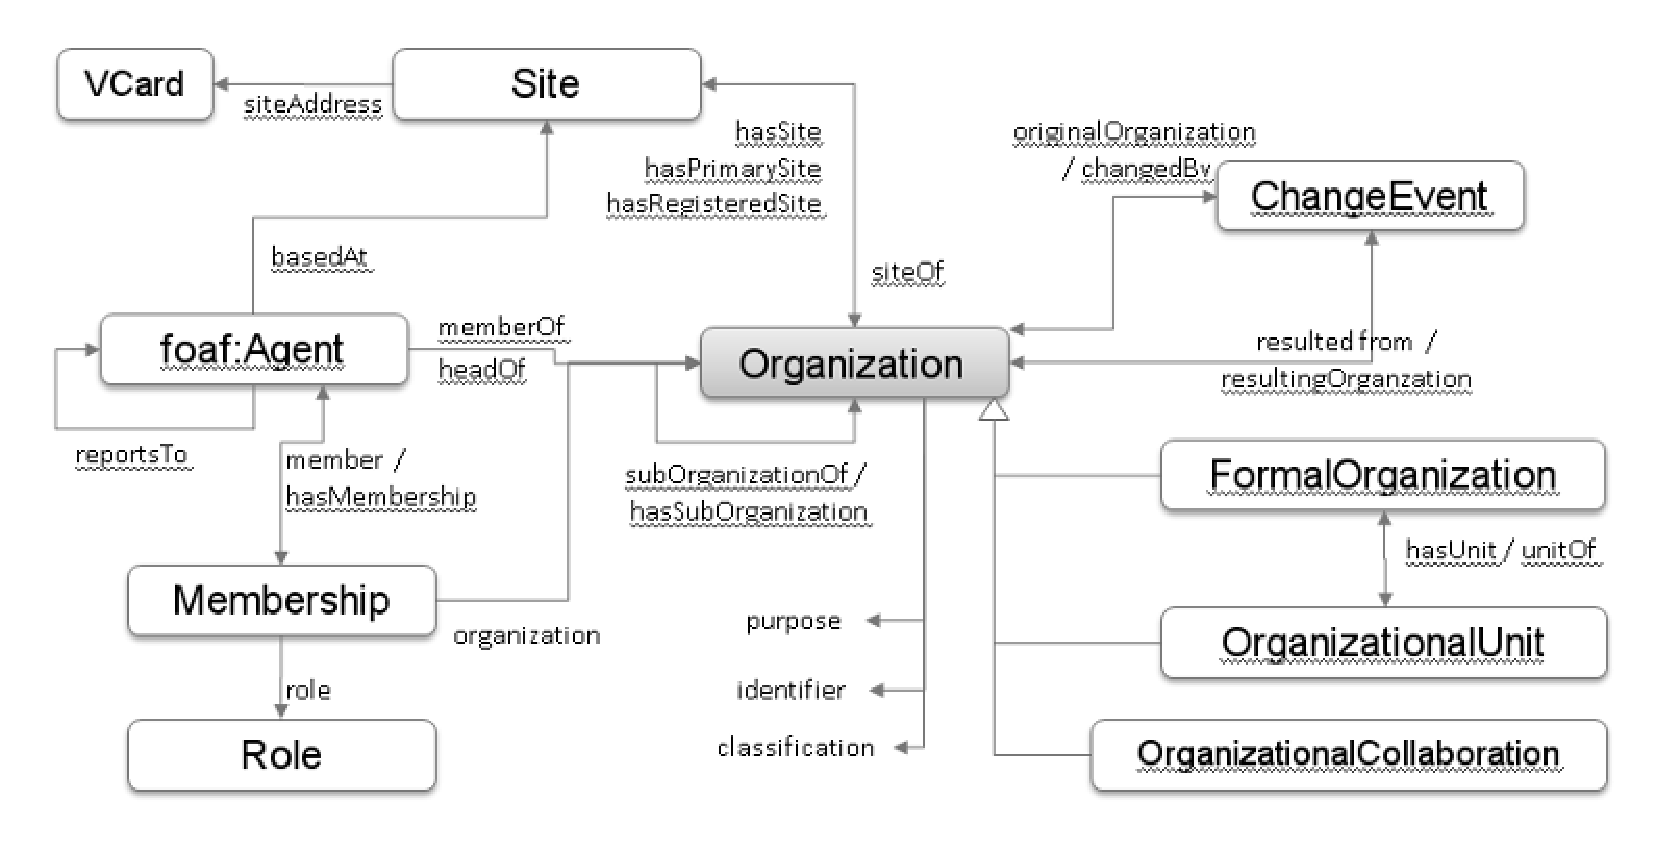
\includegraphics[width=14cm]{images/phd/org}
  \caption{\textit{Organizations Ontology. Overview.}}
 \label{fig:org-ontology}
\end{figure}

Desde otro punto de vista no tan centrado en la corriente de Web Semántica y ontologías, hay que referenciar 
la propuesta de datos abiertos realizada por \textit{OpenCorporates} a través ``\textit{The Open Database Of The Corporate World}'', han utilizado
técnicas de \textit{screen scrapping} y \textit{crawling} para extraer información de más de $12$ millones de compañías. Esta
información, ver Figura~\ref{figure:open-org}, tiene un alto valor para reutilizar y trazar la actividad de una empresa ya que disponen en la mayoría
de los casos del identificador de la empresa. La información de esta base de datos sigue un enfoque mixto entre \opendata y \linkeddata, 
pero el gran problema reside en la ausencia de un modelo formal para la descripción de los datos, es por ello que disponer de un modelo formal 
que integre esta información es clave para la posible reutilización de la información y explotación de la misma de una forma estándar.

\begin{figure}[!h]
\begin{center}
\begin{lstlisting}[language=SPARQL]
    <http://opencorporates.com/companies/nl/37136346.rdf?id=5828504>    
      a <http://purl.org/dc/dcmitype/Text>,
                foaf:Document;
         dct:format "application/rdf+xml";
         dct:isFormatOf 
	  <http://opencorporates.com/companies/nl/37136346?id=5828504>;
         dct:title "Linked Data in RDF format for Benuma";
         foaf:primaryTopic 
	  <http://opencorporates.com/id/companies/nl/37136346> .
	  ...
        <http://opencorporates.com/id/companies/nl/37136346>     
	a <http://s.opencalais.com/1/type/er/Company>;
         :label "Benuma" 
\end{lstlisting}
\caption{Información (parcial) sobre una Organización de ``Open Corporates'' en N3.}
\label{figure:open-org}
\end{center}
\end{figure}

\cleardoublepage
\subsubsection{Proyectos de Investigación}
Los proyectos de investigación de los principales programas competitivos
también se han visto involucrados en el despliegue de sistemas de contratación
pública electrónica utilizando semántica y datos enlazados. Entre ellos
se pueden destacar los siguientes:
\begin{description}
 \item [\textit{LOTED Project}~\cite{loted-project}] \textit{Linked Open Tenders Electronic Daily} realizado
por el grupo KMI de la \textit{Open University} del Reino Unido permite la consulta en \gls{SPARQL} de anuncios de licitación
publicados a través de los \gls{RSS} de \gls{TED}. Se trata del tradicional enfoque de \textit{Rdfizar}, información
ya publicada y hacerla disponible a través de un \textit{endpoint} de SPARQL. Sin duda se trata
de una importante iniciativa tanto por su carácter innovador, como por tratarse de la primera apuesta
real de utilización de semántica en los anuncios de licitación, sin embargo, tan sólo llega a los anuncios
de licitación publicados en TED y también parece que el demostrador oficial ha dejado de ser 
mantenido por los autores. No obstante, es necesario considerar esta propuesta para aprovechar
el efecto experiencia de la misma.
 \item [\textit{LOD2 Project}~\cite{lod2-project}.] Este proyecto europeo al que se ha referenciado en la
Sección~\ref{lod2-project} por su esfuerzo en la iniciativa \linkeddata desde un punto de vista genérico, también ha seleccionado la contratación pública electrónica como un caso de uso estratégico, es por ello
que han aumentado los paquetes de trabajo para incluir el esfuerzo de la \textit{Charles University} de la República Checa y su investigación sobre la aplicación de \linkeddata y semántica en el campo
del \eproc. Esto se ha manifestado en la constitución del paquete de trabajo \textit{WP9A – LOD2 for a Distributed Marketplace for Public Sector Contracts}.
La importancia del seguimiento de este proyecto reside tanto en las personas como en las instituciones implicadas, ya que generan 
una gran cantidad de tecnología y \textit{know-how} especialmente relevante para el estudio objeto de este documento y para las iniciativas
de \linkeddata y \opendata en general.
 \item [\textit{LATC Project}~\cite{latc-project}.] \textit{Linked open data around-the-clock} es un proyecto europeo,
una \textit{Specific Support Action} en el contexto del 7º Programa Marco-ICT formado por más de 58 instituciones
en los que se realizan y coordinan proyectos, personas. etc. El objetivo de este proyecto es gestionar la información
y datos generados a través de distintas fuentes proveyendo la infraestructura y documentación necesaria para
desplegar arquitecturas que den soporte a los datos enlazados. Prueba de su ingente capacidad es la cobertura y 
asesoramiento a proyectos y a investigadores de Europa (74\%) y de Estados Unidos (25\%). El consorcio
está formado por instituciones y empresas tan relevantes en este campo como: \textit{Digital Enterprise Research Institute} (DERI), \textit{NUI Galway}, Irlanda;
\textit{Vrije Universiteit Amsterdam} (VUA), Países Bajos; \textit{Freie Universit\"{a}t Berlin} (FUB), Alemania; \textit{Institute for Applied Informatics} e.V. (InfAI), Alemania y
\textit{Talis Information Ltd.}, Reino Unido.

\item [\textit{PlanetData Project}~\cite{planet-data-project}.] Se trata de una Red de Excelencia en el 
ámbito europeo (FP7-257641) con un presupuesto total de $3.72$ millones de euros y en la que participan los principales 
organismos de investigación con el objetivo de sumar los esfuerzos de la comunidad de investigadores para ofrecer 
a las organizaciones interesadas en la iniciativa de \linkeddata soporte con la publicación de sus datos. Evidentemente 
cuentan con un estrecho lazo con los proyectos anteriores y su actividad cubre las cuestiones relacionadas con datos enlazados 
en diferentes ámbitos: \textit{data streams, (micro) blog posts, digital archives, eScience resources, public sector data sets, and the Linked Open Data Cloud}.

\item [\textit{WebDataCommons.org}~\cite{web-data-commons-project}.] Es una iniciativa conjunta realizada por el grupo 
de investigación \textit{Web-based Systems Group} en la \textit{Freie Universit\"{a}t} de Berlín y el 
\textit{Institute AIFB} perteneciente al \textit{Karlsruhe Institute of Technology}, en el cual se han extraído 
y generado tripletas \gls{RDF} de más de $65$ millones de sitios web, contando un número de 
\textit{$3.2$ billion RDF quads} a fecha de febrero del año 2012, cubriendo información sobre productos, 
personas, organizaciones, lugares, eventos y recetas de cocina entre otros. Para la realización de este 
experimento se han utilizando técnicas de extracción de información de \gls{HTML} que utilizan microformatos, RDFa, etc. 
Toda esta información y datos está disponible para su descarga y uso por terceros en RDF. La importancia de este proyecto 
reside tanto en las personas y organizaciones implicadas como en la magnitud de los datos que han conseguido extraer.

\item [Otros proyectos.] Estas iniciativas trabajan con tecnología semántica y de datos enlazados en diferentes contextos suministrando servicios
a instituciones públicas o bien realizando investigación e innovación. Entre otros, se pueden citar: \gls{FP7} project SEALS (\textit{Semantic Evaluation at Large Scale}), FP7 project SpitFIRE (\textit{Semantic-Service Provisioning for the Internet of Things using Future Internet Research 
by Experimentation}), French DataLift project y Semic.EU.
\end{description}

Igualmente a nivel nacional se han impulsado diferentes iniciativas
y proyectos, como los de la República Checa y ``10ders Information Services'', que intentan elevar el significado de la información
de los anuncios de licitación utilizando tecnologías semánticas. También hay que considerar que la reutilización
de vocabularios ya establecidos e impulsados por las distintas Administración Públicas, por ejemplo la iniciativa Joinup~\cite{joinup-europe} de la Unión Europea, 
es de suma relevancia para proporcionar información utilizando datos enlazados, en este sentido todas las iniciativas y proyectos reseñados en las secciones anteriores ayudan a 
disponer de los \textit{building blocks} necesarios para afrontar la aplicación de semántica a los procesos de contratación pública electrónica.

